\section{File Structure}
\subsection{JSON structure}
The JSON files containing the configurations of the various prediction algoirthms must be structured in the following way

\subsubsection{Support Vector Machine}
\begin{itemize}
	\item \textbf{author}: file author;
	\item \textbf{version}: version of the application with the which the file was created;
	\item \textbf{algorithm}: states which algorithm was used for training, in this particular case "SVM";
	\item \textbf{date}: date on which the file was created;
	\item \textbf{predictors}: list of predictor tags;
	\item \textbf{result}: list of coefficients obtained from training.
\end{itemize}
\begin{figure}[H]
\centering
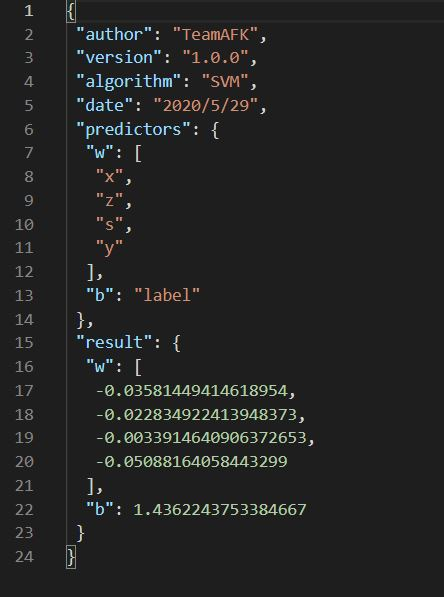
\includegraphics[scale=0.65]{img/json/jsonSVM.jpg}
\caption{Support Vector Machine JSON example}
\end{figure}
\newpage

\subsubsection{Linear Regression}
\begin{itemize}
	\item \textbf{author}: file author;
	\item \textbf{version}: version of the application with the which the file was created ;
	\item \textbf{algorithm}: states which algorithm was used for training, in this particular case "Linear Regression";
	\item \textbf{date}: date on which the file was created;
	\item \textbf{predictors}:  list of predictor tags;
	\item \textbf{result}: list of coefficients obtained from training;
	\item \textbf{line}: the equation of the Linear Regression.
\end{itemize}
\hspace{5cm}\\
\begin{figure}[H]
\centering
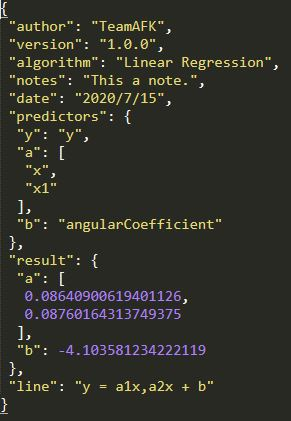
\includegraphics[scale=0.75]{img/json/jsonRL.jpg}
\caption{Linear Regression JSON example}
\end{figure}
\newpage
\subsection{CSV File structure}
The CSV files are structured based on which algorithm must be trained, RL or SVM.
Each column conains the values of the corresponding predictor\glo The first line  of each column must contain the tag associated to the particualar predictor. Depending on the case, one or more colums must be present for the predictors.

\begin{figure}[H]
\centering
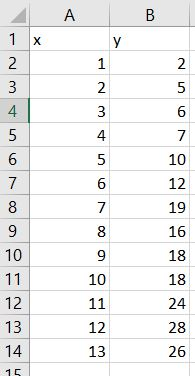
\includegraphics[scale=1]{img/json/csvfile.jpg}
\caption{CSV file example in Microsoft Excell}
\end{figure}
